\documentclass[a4paper,12pt]{report}
\usepackage{graphicx}
\usepackage{titlesec}
\titleformat{\chapter}{}{}{0em}{\bf\LARGE}
\usepackage[utf8]{inputenc}
\usepackage{url}

% Title Page
\title{Middle East Technical University\\Department of Physics\\PHYS222 Optics and Waves Laboratory\\\textbf{Experiment OW-6\\Michelson Interferometer\\Laboratory Report}}

\author{Oğuzhan ÖZCAN\\1852334\\\\Partner: İnci SAİM\\\\Teaching Assistant: Kamil ÇINAR}


\begin{document}
\maketitle
\tableofcontents
\listoffigures
\listoftables
\chapter{Theory}
There are many devices that we can observe two-beam interference. Michelson interferometer is a device that can produce two wavefronts to be physically seperated by a large distance. The two interfering wavefronts produced by the reflections from the two mirrors. At the center of the device there is a beam splitter and usually one of the face of the splitter is covered with silver. This device is developed by Albert Abraham Michelson in 1880. Michelson interferometer is used by A. A. Michelson and E. Morley in their specific experiment which is \textit{Michelson-Morley experiment} in 1887 and gave
experimental proof of the fact that the value of the speed of light was independent
of the coordinate axis and so brought a demonstration of the validity
of Einstein’s \textit{Special Theory of Relativity} [1].  
\begin{figure}[h!]
\centering
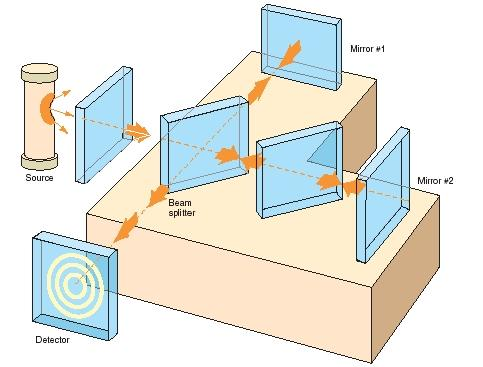
\includegraphics[width=0.75\linewidth, height=0.30\textheight]{michelson}
\caption{Michelson Interferometer}
\label{fig:michelson}
\end{figure}
Modern versions of this interferometer are widely used in spectroscopy.\\\\
The working principle of Michelson interferometer is not complicated. The interferometer is illuminated by a monochromatic source. This light ray strikes to beamsplitter directly. In this case, beamsplitter plays two roles. Firstly, it seperates the incident beam into two identical beams and these beams are send to \textit{Mirror 1} and \textit{Mirror 2.}Secondly, then beamsplitter recombines these beams so that thay interfere on a screen. Obviously, the purpose of this device is the observing fringes with a low order of interference. At this point we have to define the importance of Mirror 1. Note that the beams which is reflected by Mirror 1 makes an extra double transit inside the beam splitter. Because of this effect we can insert a fourth plate which is known as \textit{compensator plate} in front of the Mirror 2 [2]. A compensator plates almost same with beamsplitter. Only difference is that a compensator plates is antireflection coated on both sides.\\\\
As we mentioned above, Michelson-Morley experiment is crucial for Einstein's theory of special relativity. Many scientists worked for define the speed of light. In 1862, French physicist L\'{e}on Foucault defined the best value for speed of light in air as 298000$\pm$500 km/sec by using rotating mirror. In 1882, Newcomb defined the speed of light as 299860$\pm$30 km/sec. Most precise experiment was done by Michelson and Morley. They defined the speed of light as 299796$\pm$4 km/sec [3]. 






















































\chapter{Data and Results}
\section{Measurement of the Laser Wavelength}
\begin{table}[h]
	\begin{center}
\begin{tabular}{|c|c|c|c|}
	\hline $d_{i}$ & 60 $\mu m $ & 60 $\mu m $ & 60 $\mu m $ \\ 
	\hline $N_{i}$ & 191 & 189 & 192 \\ 
	\hline $\lambda_{i}$ & 628.3 nm & 634.9 nm & 625.0 nm \\ 
	\hline 
\end{tabular} 
\end{center}
\caption{Sample data for wavelength} 
\end{table}
\textbf{1. Calculate $\lambda_{i}$ for each trial.}
\begin{center}
	{\Large $\lambda=\frac{2d\cdot n}{N}$}
\end{center}
\begin{center}
$\lambda_{i,1}=\frac{2\cdot60\times10^{-6}\cdot 1}{191}=628.3$nm
\end{center}
\begin{center}
	$\lambda_{i,2}=\frac{2\cdot60\times10^{-6}\cdot 1}{189}=634.9$nm
\end{center}
\begin{center}
$\lambda_{i,3}=\frac{2\cdot60\times10^{-6}\cdot 1}{192}=625.0$nm
\end{center}
\textbf{2. Calculate from these results an average value and a standard deviation for the laser wavelength $\lambda$.}\\
Average wavelength $\bar{\lambda}$ can be determine by using following equation
\begin{center}
{\Large 	$\bar{\lambda}=\frac{\lambda_{i,1}+\lambda_{i,2}+\lambda_{i,3}}{3}$}
\end{center}
Therefore, average wavelength $\bar{\lambda}$ will be
\begin{center}
	{\Large 	$\bar{\lambda}=\frac{628.3+634.9+625.0}{3}$}
\end{center}
\begin{center}
	{\Large 	$\bar{\lambda}=629.4$ nm}
\end{center}
Standard deviation of wavelength, $\Delta \lambda$, can be determine by using following equation
\begin{center}
	{\Large $\Delta \lambda=\sqrt{\sum_{i=1}^{m}\frac{(\lambda_{i,m}-\bar{\lambda})^{2}}{m-1}}$}
\end{center}
Therefore, in our case, standard deviation will become
\begin{center}
	{\Large $\Delta \lambda=\sqrt{\frac{(628.3-633.0)^{2}+(634.9-633.0)^{2}+(625.0-633.0)^{2}}{2}}$}
\end{center}
\begin{center}
	{\Large $\Delta \lambda=6.7$ nm}
\end{center}
After finding standard deviation we can determine our error range. To determine the error range following equation will be useful
\begin{center}
{\large 	$\lambda=\bar{\lambda}\pm\Delta \lambda$}
\end{center}
Therefore, in our experiment we will have
\begin{center}
	$\lambda$=629.4 nm $\pm$ 6.7 nm = 622.7 nm, 636.7 nm
\end{center}
\textbf{3. Is your result in agreement with the specified value of $\lambda$= 633.0 nm within the error limits of the measurement?}\\
When we compare the result that we obtain in 2.1.1 and 2.1.2, we can say with no dubt our results are agree with the theoretical value. We can also check percentage error of the experiment to determine the validity of experimental data.
\begin{center}
	Percentage Error = $\frac{|Theoretical Value-Experimental Value|}{Theoretical Value}\times 100\%$
\end{center}
\begin{center}
	Percentage Error = $\frac{|633.0-629.4|}{633.0}\times 100\%$
\end{center}
\begin{center}
	Percentage Error = $0.5\%$ nm
\end{center}
\textbf{4. Derive $N\lambda=2 n d$}\\
Let assume that waves whose are reflected by Mirror 1 and at angle of $\theta$ to the z-axis by Mirror 2. The resulting plane waves will be 
\begin{center}
	$E_{1}=E_{0}\exp i [k(z+2\Delta d)-\omega t]$ \\
$E_{2}=E_{0}\exp i [kz\cos\theta+kx'\sin\theta-\omega t]$
\end{center}
In the region where two beams overlap, the resultant electric field is
\begin{center}
	$E_{tot}=E_{1}+E_{2}$\\
$E_{tot}=E_{0}e^{-i\omega t}(\exp[ik+(z+2\Delta d )]+\exp[ikz\cos\theta+kx'\sin\theta])$
\end{center}
The intensity can now calculated using
\begin{center}
	$I_{tot} \sim E_{tot}\cdot E_{tot}^{*}$
\end{center}
which yields the result
\begin{center}
	$I_{tot}=4 I_{0}\cos^{2}k(\Delta d-\frac{x'}{2}\sin\theta+z\sin^{2}\frac{\theta}{2})$
\end{center}
Therefore, for fixed $\Delta d $, we have fringes at intervals $\Delta x'$ given by
\begin{center}
	$\Delta x'=2 \lambda/\sin\theta$
\end{center}
When Mirror 1' is moved in a direction normal to its face, the fringe pattern moves as $\Delta d$
changes. The number, $n$, of the fringes that cross the center of the screen when Mirror 2 is moved a
distance  $\Delta d$ is given by
\begin{center}
	$n\lambda=2\Delta d$ 
\end{center} 
Now can calculate the fringe radii by considering a point P lying on a circular fringe. The
optical path difference at $P$ is $\delta=(R_{1}-R_{2})=2\Delta d\cos\theta$. The point $P$ lies on a bright fringe if
$\delta=n\lambda$ (\textit{n} is called the order of the fringe). The polar angle, $\theta_{n}$, where the \textit{n-th} order fringe occurs
is given by
\begin{center}
	$2\Delta d\sin\theta_{n}=n\lambda$
\end{center}
\textbf{5. Your apparatus have not contained a compensator plate. What effect does this have on your results? Explain the purpose of a compensator plate and why it might be essential for certain measurements.}\\
When there is a compensator plate, each beam will pass through equal thickness of glass. The compensator plate is an exact duplicate of beamsplitter. Note that there is an exception for silver coated and thin film coated beamsplitters. A compensator plate usually oriented at angle of $45^{\circ}$. If there is a compensator plate then any optical path differences arises from the actual path difference. As we know the dispersion of the beamsplitter causes to an optical path which is a function of $\lambda$. Note that the inclusion of compensator plate decreases the effects of dispersion [4]. 
\newpage 
\section{Measurement of the Refractive Index}
\begin{table}[h!]
	\begin{center}
\begin{tabular}{|c|c|c|c|}
	\hline $\Delta P_{i}=P_{final}-P_{initial}$ & 70 kPa & 70 kPa & 70 kPa \\ 
	\hline $N_{i}$ & 19 & 21 & 19 \\ 
	\hline $n_{air,i}$ & 1.000000003 & 1.000000003 & 1.000000003 \\ 
	\hline 
\end{tabular}
\end{center}
\caption{Sample data for refractive index of air} 
\end{table}
\textbf{1. Calculate $n_{air}$ for each trial.}\\
Refractive index of air can be determine by following equation
\begin{center}
	{\Large $n_{atm}=1+(\frac{N}{\Delta P})(\frac{\lambda}{2d})P_{atm}$}
\end{center}
Note that in the above equation refractive index of air is given with respect to atmosferic pressure. However, in the experiment we have used Pascal (1 atm=101325 Pa). Therefore, measured refractive indices will be
\begin{center}
	{\large $n_{atm,1}=1+(\frac{19}{70\times10^{3}Pa})(\frac{633.0\times10^{-9}m}{2\cdot31\times10^{-3}m})\cdot101325$ Pa}
\end{center}
\begin{center}
$n_{atm,1}\cong1.000000003$
\end{center}
\begin{center}
	{\large $n_{atm,2}=1+(\frac{21}{70\times10^{3}Pa})(\frac{633.0\times10^{-9}m}{2\cdot31\times10^{-3}m})\cdot101325$ Pa}
\end{center}
\begin{center}
	$n_{atm,2}\cong1.000000003$
\end{center}
\begin{center}
	{\large $n_{atm,3}=1+(\frac{19}{70\times10^{3}Pa})(\frac{633.0\times10^{-9}m}{2\cdot31\times10^{-3}m})\cdot101325$ Pa}
\end{center}
\begin{center}
	$n_{atm,3}\cong1.000000003$
\end{center}
\textbf{2. Calculate from these results, an average value and a standart deviation for refractive index of air.}\\
We can obtain an average value by using following equation
\begin{center}
	$\bar{n}=\frac{n_{air,1}+n_{air,2}+n_{air,3}}{3}$
\end{center}
\begin{center}
	$\bar{n}=\frac{1.000000003+1.000000003+1.000000003}{3}$
\end{center}
\begin{center}
	$\bar{n}=1.000000003$
\end{center}
Then we can obtain standard deviation by using following equation
\begin{center}
	{\Large $\Delta n_{air}=\sqrt{\sum_{i=1}^{m}\frac{(n_{air,i}-\bar{n})^{2}}{m-1}}$}
\end{center}
Therefore, standard deviation will be, in this case
\begin{center}
	{\large $\Delta n_{air}=\sqrt{\frac{(1.0-1.000000003)^{2}+(1.0-1.000000003)^{2}+(1.0-1.000000003)^{2}}{2}}$}
\end{center}
\begin{center}
	{\large $\Delta n_{air}=0.000000003$}
\end{center}
After obtaining standar deviation we can determine error range by using following equation
\begin{center}
	$n_{air}=\bar{n}\pm\Delta n$
\end{center}
\begin{center}
	$n_{air}=1.000000003\pm 0.000000003$
\end{center}
\begin{center}
	$n_{air}=1.000000000, 1.000000006$
\end{center}
\textbf{3. Compare your result to the literature value.}\\
As we know, refractive index of air is 1.000000000. In the experiment, we found the refractive index of air as 1.000000003. As seen, there is a very little error. By calculating percentage error we can say that our values are valid.
\begin{center}
	Percentage Error=$\frac{|1.000000000-1.000000003|}{1.000000000}\times100\%$
\end{center}
\begin{center}
	Percentage Error = .0000003$\%$
\end{center}
\textbf{4. Derive $n_{atm}-1=(N/\Delta P)(\lambda/2d)P_{atm}$}\\
\textit{(Hint: Assume that the amount by which $n_{air}$ is greater than 1 depends linearly on pressure. Thus if $n_{air}$ at $P_{atm}$ is $1+\delta$, it becomes $1+\delta/2$ at half the $P_{atm}$ pressure)}\\
The index of a medium is 
\begin{center}
	$n=\frac{c}{v}$
\end{center}
In a vacuum, $v=c$, so $n$ is exactly 1. For gases, the index of refraction increases linearly with pressure. This phonemena can be expressed as
\begin{center}
	$n-1=P\frac{dn}{dP}$
\end{center}
Then we can simply have to find the rate of change of the $n$ with respect to pressure, $P$. When we mount a vacuum pump in front of the Mirror 2, we can change the pressure. In this case the wavelength of the light in a medium index of refraction $n$ is
\begin{center}
	$\lambda=\frac{\lambda_{0}}{n}$
\end{center}
where $\lambda_{0}$ is the wavelength in vacuum. Recall that when a wave traverses a distance $x$,
its phase changes by
\begin{center}
	$\Delta\phi=\frac{2\pi x}{\lambda}$
\end{center}
In this case, if the thickness of the cell is $t$, since the light travels through it twice, the
phase shift for constant $n$ would be
\begin{center}
	$\Delta\phi=\frac{2\pi2t}{\lambda_{0}/n}=\frac{4\pi nt}{\lambda_{0}}$
\end{center}
So, with the cell in place, with atmospheric pressure, we have a certain fringe pattern.
When the air is pumped out, there are $N$ fringe transitions, one for each phase shift of $2\pi$. For a net change, $\Delta n$, in the index of refraction, the above equation gives
\begin{center}
	$\frac{2\pi2t\Delta n}{\lambda_{0}}=2\pi N$
\end{center}
so
\begin{center}
	$\Delta n =\frac{N\lambda_{0}}{2t}$
\end{center}
and
\begin{center}
	$\frac{dn}{dP}\approx\frac{\Delta n}{\Delta P}=\frac{N\lambda_{0}}{2t\Delta P}$
\end{center}
And so, finally
\begin{center}
	$n-1=\frac{P_{A}N\lambda_{0}}{2t\Delta P}$
\end{center}
where $P_{A}$ is the atmosferic pressure, $\lambda_{0}$ is the light wavelength, and $t$, the thickness of the vacuum chamber.

\chapter{Discussion and Conclusion}
\textbf{1.What are the possible errors in the experiment?}\\
Experiment setup was very sensitive. That is why we have some human based error while rotating the mirror. We can also have some error while caunting the fringes which is produced by laser. In the second part of the experiment, we did not have digital barometer so pressure in the medium may calculated with some error.\\\\
\textbf{2.What kind of approximation did you take into consideration while you were obtaining the physical quantities and how do they affect your results?}\\
While observing the fringes we only considered the bright fringes and we made our calculations by ignoring dark fringes. We took an approximate wavelength for laser. In the second part of the experiment, we took an approximate value for pressure because barometer was not digital and the needle of the barometer was so sensitive.\\\\ 
\textbf{3.What discrepancies did you encounter between the calculated quantities and theoretical or literature values?}\\
Obviosuly, we do not have certain discrepancies in our experiment. In the first part of the experiment, we found the wavelength of the laser at a valid gap according to theoretical values. In the second part of the experiment, we measured the refractive index of air with an error of 1/1000000000.\\\\
\textbf{4.What is your overall conclusion?}\\
To sum up, in this experiment another application of interference of light is well studied. We investigated another interference phonemena which is Michelson Interferometer. As we mentioned in the theory part of the laboratory report, Michelson's experiment which is co-operated with Morley is a proof of Einstein's theory of special relativity.  
\chapter{Application}
\textbf{Virgo Interferometer}\\
The VIRGO is a gravitational wave detector in Italy, which started operating in 2007. It is one of a handful of the world's major experiments working towards the observation of gravitational waves. VIRGO is located within the site of EGO (European Gravitational Observatory) at Santo Stefano a Macerata, Cascina, Tuscany.\\\\
VIRGO is a Michelson laser interferometer with two orthogonal arms each 3 kilometers long. A beam splitter divides the incident laser beam into two equal components sent into the two arms of the interferometer. In each arm, a two mirrors Fabry-Perot resonant cavity extends the optical length from 3 to about 100 kilometers because of multiple reflections and therefore amplifies the tiny distance variation caused by a gravitational wave. The two beams of laser light coming from the two arms, are recombined out of phase on a detector so that, in principle, no light reaches the detector. The variation of the optical path’s length, caused by the changing distance between the mirrors, produces a very small phase shift between the beams and, thus, a variation of the luminous intensity, which is proportional to the wave’s amplitude.\\\\
However, in this scheme, a large fraction of the light is sent back toward the laser. In order to further increase the power, this light is sent back to the interferometer by a recycling mirror, in phase with the incident beam thus increasing the light power that can reach several tens of kilowatts in the Fabry-Perot resonant cavities. A high light power is important because it allows to improve the sensitivity of the interferometer. With these resonant cavities coupled together, the interferometer can be seen as a giant light trap. If the optics would be perfect and the mirrors perfectly stable, no light should normally reach the detector except when the interferometer plane is crossed by a gravitational wave. The quality and stability of the optics represent therefore one of the major challenges of the interferometer.\\\\ 
VIRGO is sensitive to gravitational waves in a wide frequency range, from 10 to 10,000 Hz. This should allow the detection of gravitational radiation caused by the coalescence of binary systems (stars or black holes), pulsars and those produced by supernovae in the milky way and in outer galaxies, for instance from the Virgo cluster, hence the name of the project.\\\\ 
VIRGO runs day and night, listening to all signals that arrive at any time from any part of the universe. The data cominig from the interferometer as well as the ancillary data necessary to its control (4Mbytes/s) are subjected to a preliminary analysis for quality check and a quick detection of potentially interesting anomalous signals. The data is then put at the disposal of the scientific collaboration, for a deeper analysis [5].
\chapter{References}
$[1]$ Kenyon, I. (2008). \textit{The Light Fantastic: A Modern Introduction to Classical and Quantum Optics} (p. 103). Oxford England: Oxford University Press.\\
$[2]$  Chartier, G. (2005). \textit{Introduction to Optics} (p. 276). New York: Springer.\\
$[3]$ Flügge, S. et al. (Ed.). (1956). \textit{Handbuch der Physik-Encyclopedia of Physics} (Vol. XXIV, p. 7.8.9). Berlin: Springer-Verlag.\\
$[4]$Interferometer for the detection of gravitational waves. (n.d.). Retrieved May 8, 2015, from http://www.ego-gw.it/virgodescription/pag-3.html






















\end{document}          
